\documentclass[conference]{IEEEtran}
\IEEEoverridecommandlockouts
% The preceding line is only needed to identify funding in the first footnote. If that is unneeded, please comment it out.
\usepackage{cite}
\usepackage{amsmath,amssymb,amsfonts} % 用于数学公式和符号
\usepackage{algorithm}
\usepackage{minted}         % 用于代码高亮
\usepackage[noend]{algpseudocode} % 与algorithm包配合使用，定义算法环境样式
\usepackage{caption}        % 更好地控制图表标题
\usepackage{hyperref}       % 用于生成超链接，方便引用
\usepackage{float}
\usepackage{stfloats}
\usepackage{graphicx}
\usepackage{textcomp}
\usepackage{xcolor}
\usepackage{array}
\usepackage{stfloats}
\usepackage{booktabs}
\usepackage{longtable}
\usepackage{tabularx}
\usepackage{multirow}
\usepackage{makecell}
\usepackage{tabularx}   % 【核心】用于创建自适应宽度的表格
\usepackage{ragged2e}   % 用于更美观的左对齐（\RaggedRight）
\usepackage{subcaption} % 用于创建带标签的子图环境
\usepackage{caption}    % 建议同时使用，以获得更好的标题控制
\def\BibTeX{{\rm B\kern-.05em{\sc i\kern-.025em b}\kern-.08em
    T\kern-.1667em\lower.7ex\hbox{E}\kern-.125emX}}
\begin{document}

\title{A Multi-Segment Logarithmic Spiral Continuum Robot with a Stretchable Central Backbone: Design and Coupled Kinematic Modeling}

\author{\IEEEauthorblockN{1\textsuperscript{st} Huaicheng Huang}
\IEEEauthorblockA{\textit{University of Bristol}\\
\textit{School of Electrical, Electronic}\\ \textit{and Mechanical Engineering}\\
Bristol, UK}
~\\
\and
\IEEEauthorblockN{2\textsuperscript{nd} Guolei Wang}
\IEEEauthorblockA{\textit{Department of Mechanical Engineering} \\
\textit{Tsinghua University}\\
Beijing, China}
*Corresponding author
~\\
\and
\IEEEauthorblockN{3\textsuperscript{rd} Ken Chen}
\IEEEauthorblockA{\textit{Department of Mechanical Engineering} \\
\textit{Tsinghua University}\\
Beijing, China}

}

\maketitle

\begin{abstract}
This paper introduces a new four-segment continuum robot inspired by the biological structure of a logarithmic spiral. The robot is characterized by its stretchable elastic backbone and segment-based actuation. We developed a detailed coupled kinematic model based on an enhanced piecewise constant curvature (PCC) framework, which incorporates dynamic compensation for backbone length and a systematic analysis of coupling effects. This allows for mapping high-level shape commands directly to actuator controls. A 12-DoF physical prototype was constructed to validate our model experimentally. The qualitative results demonstrate the robot's extensive workspace and its remarkable ability to achieve complex configurations, including S-shapes and spatial spirals, confirming the design's high flexibility. Furthermore, quantitative analysis verifies the model's predictive accuracy for the robot's structure in open-loop scenarios, setting the stage for future work on model-based dynamic and closed-loop control.
\end{abstract}

\begin{IEEEkeywords}
Continuum Robotics, Logarithmic Spiral Robot, Kinematic Modeling
\end{IEEEkeywords}

% ===========================
% === Secion I: Introduction
% ===========================

\section{Introduction}
Bio-inspiration has always been a core driving force in the development of continuum robots. However, to achieve the versatile bending and twisting configurations of a logarithmic spiral continuum robot, we developed a novel inverse kinematic model based on length, which fully utilizes the mathematical properties of the logarithmic spiral. The concept of bio-inspired continuum robots based on the logarithmic spiral was proposed by Wang et al. \cite{b1}, but their work did not further elaborate on the associated kinematics. In the related literature on logarithmic spiral continuum robots, there are no reported cases of segmental actuation \cite{b2}. And the derivation process for improved variable-curvature designs in forward kinematics is extremely complex \cite{b3}. Other modeling techniques, such as beam theory (including Cosserat rod theory \cite{b4}\cite{b5}) and the Finite Element Method (FEM) \cite{b6}, offer higher accuracy by analyzing forces and strain energy. However, these methods demand significant computational resources, making them difficult to use for real-time applications. 

Although the Piecewise Constant Curvature (PCC) model is a simplified approach for continuum robot kinematics, it demonstrates excellent robustness when applied to our segmental logarithmic spiral robot structure. This approach also reduces derivation complexity by focusing on inverse kinematics. The resulting segmentally actuated logarithmic spiral continuum robot exhibits excellent stability at its base, flexibility at its tip, and favorable motion characteristics in its intermediate segments.

The paper is organized as follows. Section II outlines the robot's mechanical design. It provides an in-depth explanation of our proposed coupled kinematic model, including its inverse kinematics and the forward kinematics used for validation. Section III presents the experimental results for the model's validation. Finally, Section IV concludes the paper and outlines future work.

% =====================
% === Secion II: Method
% =====================

\section{Method}
This section describes the core technology of our proposed multi-segment logarithmic spiral continuum robot. We will first introduce the robot's mechanical design, highlighting the novelty of its structure. We will then derive its kinematic model in detail, providing a theoretical foundation for subsequent simulation and control.

\subsection{Mechanical Design}
We designed and constructed a four-segment logarithmic spiral continuum robot with a total length of 80 cm (Fig. 1A). The core of its design lies in its bio-inspired joint layout and a stretchable backbone.

% ===============================================
%    Combination Figure: Robot Design Showcase
% ===============================================
\begin{figure*}[t]
    \centering
    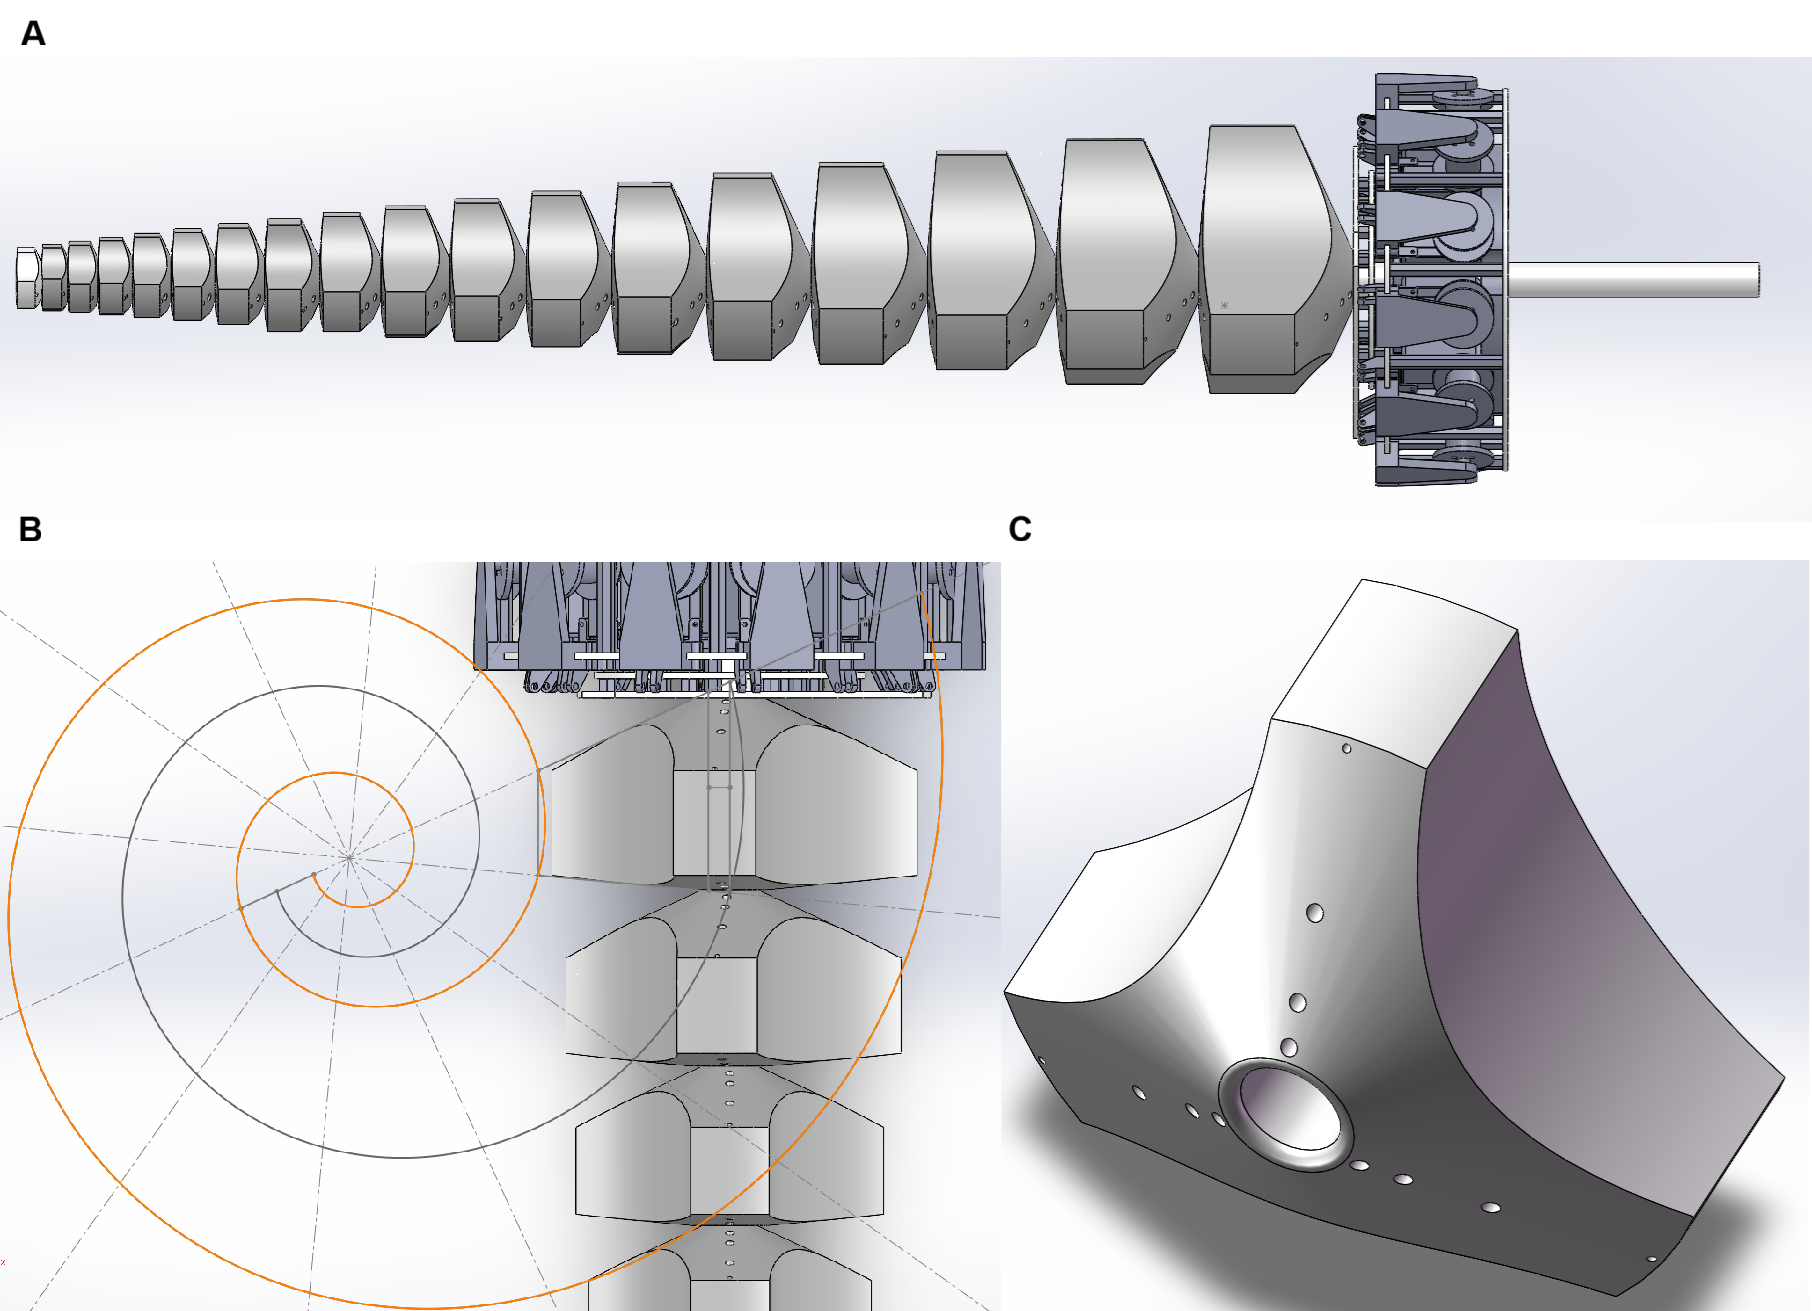
\includegraphics[width=\textwidth]{assets/Method.png}
    \caption{Demonstration of the logarithmic spiral design concept and the robot prototype's motion capabilities. (A) The four-segment logarithmic spiral continuum robot prototype. (B) A schematic of the logarithmic spiral design concept. The orange curve represents the standard logarithmic spiral, $\rho(\theta) = a \cdot e^{b \theta}$. (C) A model of a single joint, the 18th joint.}
    \label{fig:spiral_diagram}
\end{figure*}
% ===============================================

\subsubsection{Logarithmic Spiral Joints and Stiffness Gradient}
The placement of the outer boundaries for the robot's discrete joints is strictly governed by the logarithmic spiral equation \eqref{eq:spiral} (Fig. 1B). This design results in smooth, variable-curvature bending.

\begin{equation}
    \rho(\theta) = a \cdot e^{b \theta}
    \label{eq:spiral}
\end{equation}

Following the work of Wang et al. \cite{b1}, the logarithmic spiral function for its stretchable central backbone, is given by equation \eqref{eq:spiral_central}.

\begin{equation}
    \rho_c(\theta) = \frac{1}{2}\left(a e^{b(\theta+2\pi)} + a e^{b\theta}\right) = \frac{a}{2}\left(e^{2\pi b} + 1\right)e^{b\theta}
    \label{eq:spiral_central}
\end{equation}

Furthermore, a constant scaling factor exists between adjacent joints, as shown in equation \eqref{eq:beta_factor}. This allows the entire structure to be generated by scaling a single base unit, which greatly simplifies the manufacturing process. 

\begin{equation}
    \beta_{factor} = e^{(b\Delta\theta)}
    \label{eq:beta_factor}
\end{equation}

\subsubsection{Stretchable Central Elastic Backbone and Actuation}

The robot's central backbone incorporates a continuous spring tube with initial tension. Its ability to stretch axially allows it to passively accommodate the changing geometric arc length during different bending poses, thereby preventing the buckling issues common in rigid skeletons. Additionally, the hollow design of the spring tube provides a channel for tool or sensor integration.

The entire robot is actuated by 12 servo motors via Dyneema cables in a differential drive configuration to achieve joint bending. As shown in Fig. 1C, these cables are routed through the central plane of each "wing" at a single joint.

\subsection{Kinematic Modeling}
The cables that actuate the distal segments originate from the motors and route sequentially through all preceding segments. This layout introduces inter-segment coupling effects and also has a stretchable central backbone. These characteristics represent the core challenge that our kinematic model needs to solve. Our primary method is to establish a coupled inverse kinematic model for the robot. The goal of this model is to compute the required step displacements for the 12 servo motors based on high-level shape commands, given as $(\phi, \theta)$.

\subsubsection{Physically-Realistic Coupled Inverse Kinematic Model}
To precisely control the bending pose of each robot segment, we developed a coupled inverse kinematic model that contains ideal logarithmic spiral geometry, physical measurements, and dynamic backbone length compensation. This model can resolve the high-level shape commands $(\phi, \beta)$ into the required step displacements for the 12 low-level servo motors.

Based on the principle that all joints are generated by scaling a single base unit, we input the ideal bent length of the base unit's backbone and its CAD-designed length into $d_{set}$. We then use equation \eqref{eq:L_ideal} to calculate $L_{ideal}$ and $L_{actual}$ for the $i$-th segment.
\begin{equation}
    L_{\text{central}} = \sum_{i=0}^{n-1} \left( d_{\text{set}} \cdot \beta_{\text{factor}}^i \right)
    \label{eq:L_ideal}
\end{equation}

The minimum cable length ($L_{min}$) achievable at the maximum bending state is derived geometrically, as shown in Eq. \eqref{eq:L_min_rope}.
\begin{equation}
    L_{\text{min}} = \frac{a\sqrt{b^2 + 1}}{b} \left( e^{b \cdot \theta_{\text{end}}} - e^{b \cdot \theta_{\text{start}}} \right)
    \label{eq:L_min_rope}
\end{equation}

The maximum bending angle for each segment is $\theta_{max}$. Equation \eqref{eq:delta_L_max} defines the actuation contraction range, $\Delta L_{contract}$, for a given bending angle, $\theta_{bend}$.
\begin{equation}
    \Delta L_{\text{contract}} = \frac{\theta_{\text{bend}}}{\theta_{\text{max}}} \cdot \left( L_{\text{ideal}} - L_{\text{min}} \right)
    \label{eq:delta_L_max}
\end{equation}

Due to stretchable central elastic backbone, a noticeable stretching effect occurs during bending; that is, the backbone length of each segment increases with its degree of bending. We use a linear interpolation formula, Eq. \eqref{eq:L_dyn}, to approximate this physical phenomenon.
\begin{equation}
    L_{\text{dyn}} = L_{\text{actual}} + \frac{\theta_{\text{bend}}}{\theta_{\text{max}}} \cdot \left( L_{\text{ideal}} - L_{\text{actual}} \right)
    \label{eq:L_dyn}
\end{equation}

Therefore, the required length of the primary contracting cable, $L_{\text{rope}}$, is jointly determined by the cable's routing angle, $\phi_{\text{rope}}$; the segment's dynamic length, $L_{\text{dyn}}$; and the bending command ($\Delta L_{\text{contract}}$, $\phi_{\text{bend}}$), as described in equation \eqref{eq:L_rope}.
\begin{equation}
    L_{\text{rope}} = L_{\text{dyn}} - \Delta L_{\text{contract}} \cdot \cos(\phi_{\text{rope}} - \phi_{\text{bend}})
    \label{eq:L_rope}
\end{equation}

Following the work of R. J. Webster III and B. A. Jones \cite{b7}, we can determine the required length for each of the three cables actuating a single joint via equation \eqref{eq:L_rope_all}. In this formula, the ideal backbone length of each segment, $L_{ideal}$, serves as the average value.
\begin{equation}
    L_{ideal} = \frac{L_{rope_1} + L_{rope_2} + L_{rope_3}}{3}
    \label{eq:L_rope_all}
\end{equation}

% ===============================================
%                    Equation 11
% ===============================================
\begin{figure*}[b]
% \hrulefill % 可选：在公式上下方添加一条水平线，使其与正文分离得更清晰
\begin{equation}
    ^{i-1}\mathbf{T}_i = 
    \begin{bmatrix}
        c_\phi^2 c_\theta + s_\phi^2 & c_\phi s_\phi (c_\theta - 1) & c_\phi s_\theta & R_i c_\phi (1 - c_\theta) \\
        c_\phi s_\phi (c_\theta - 1) & s_\phi^2 c_\theta + c_\phi^2 & s_\phi s_\theta & R_i s_\phi (1 - c_\theta) \\
        -c_\phi s_\theta & -s_\phi s_\theta & c_\theta & R_i s_\theta \\
        0 & 0 & 0 & 1
    \end{bmatrix}
    \label{eq:T_matrix}
    \tag{11}
\end{equation}
% \hrulefill % 可选的下方水平线
\end{figure*}
% ===============================================

To achieve global pose control for the four segments, we address the kinematic coupling from the proximal to the distal segments using linear superposition. The $\Delta S(k \to j, i)$ represents the displacement induced on the $i$-th cable of segment $j$ by the active bending of segment $k$. The total required displacement $\Delta S_{\text{total}}(j, i)$ for actuator $(j, i)$ is the sum of its own actuation ($k=j$) and the coupling effects from all preceding segments ($k<j$), as shown in equation \eqref{eq:coupling}.
\begin{equation}
    \Delta S_{\text{total}}(j, i) = \underbrace{\Delta S(j \to j, i)}_{\text{Self-segment movement}} + \underbrace{\sum_{k=1}^{j-1} \Delta S(k \to j, i)}_{\substack{\text{The sum of all preceding} \\ \text{segments coupling effects}}}
    \label{eq:coupling}
\end{equation}

\subsubsection{Forward Kinematic Model for Validation}
To validate our inverse kinematic model, we employ the standard Piecewise Constant Curvature (PCC) forward kinematic model as presented by Webster, R. J. and Jones, B. A.\cite{b7}. We attach a local coordinate frame $\{\mathcal{S}_i\}$ to the end of the $i$-th segment. The pose transformation from $\{\mathcal{S}_{i-1}\}$ to $\{\mathcal{S}_i\}$ is described by the homogeneous transformation matrix in equation \eqref{eq:T_matrix}, where c and s represent cos and sin, respectively. This matrix is a function of the bending parameters $(\phi_i, \theta_i)$ and the arc length $L_i$ (see Appendix for details).

The kinematic parameters for each segment are listed in Table \ref{tab:kinematic_params}.

% ===============================================
%                     Table 1
% ===============================================
\begin{table}[h]
    \caption{The kinematic parameters for each segment}
    \label{tab:kinematic_params}
    \centering
    \begin{tabular}{cccc}
        \toprule
        \textbf{Segment} & $\boldsymbol{L_{actral}}$ \textbf{(mm)} & $\boldsymbol{L_{ideal}}$ \textbf{(mm)} & $\boldsymbol{\theta_{max}}$ \textbf{(deg)} \\
        \midrule
        $1^{st}$ & 244.76 & 268.53 & 90.0 \\
        $2^{nd}$ & 223.54 & 259.73 & 120.0 \\
        $3^{rd}$ & 174.87 & 215.03 & 150.0 \\
        $4^{th}$ & 114.47 & 155.82 & 180.0 \\
        \bottomrule
    \end{tabular}
\end{table}
% ===============================================

The robot's global pose is obtained through the serial product of the transformation matrices. The total transformation from the base frame $\{\mathcal{G}\}$ to the tip of the $k$-th segment, $\{\mathcal{S}_k\}$, is given by: 
\begin{equation}
    {^\mathcal{G}\mathbf{T}_k} = \prod_{i=1}^{k} {^{i-1}\mathbf{T}_i}
    \label{eq:T_global}
    \tag{12}
\end{equation}

The position vector of the tip, $\mathbf{P}_k$, can be directly extracted from ${^\mathcal{G}\mathbf{T}_k}$.

% =====================================================
% === Secion III: Experimental Validation and Discussion
% =====================================================

\section{Experimental Validation and Discussion}

\subsection{Experimental Setup}

% ===============================================
%     Figure 2: Experimental setup
% ===============================================
\begin{figure}[htbp]
\centering{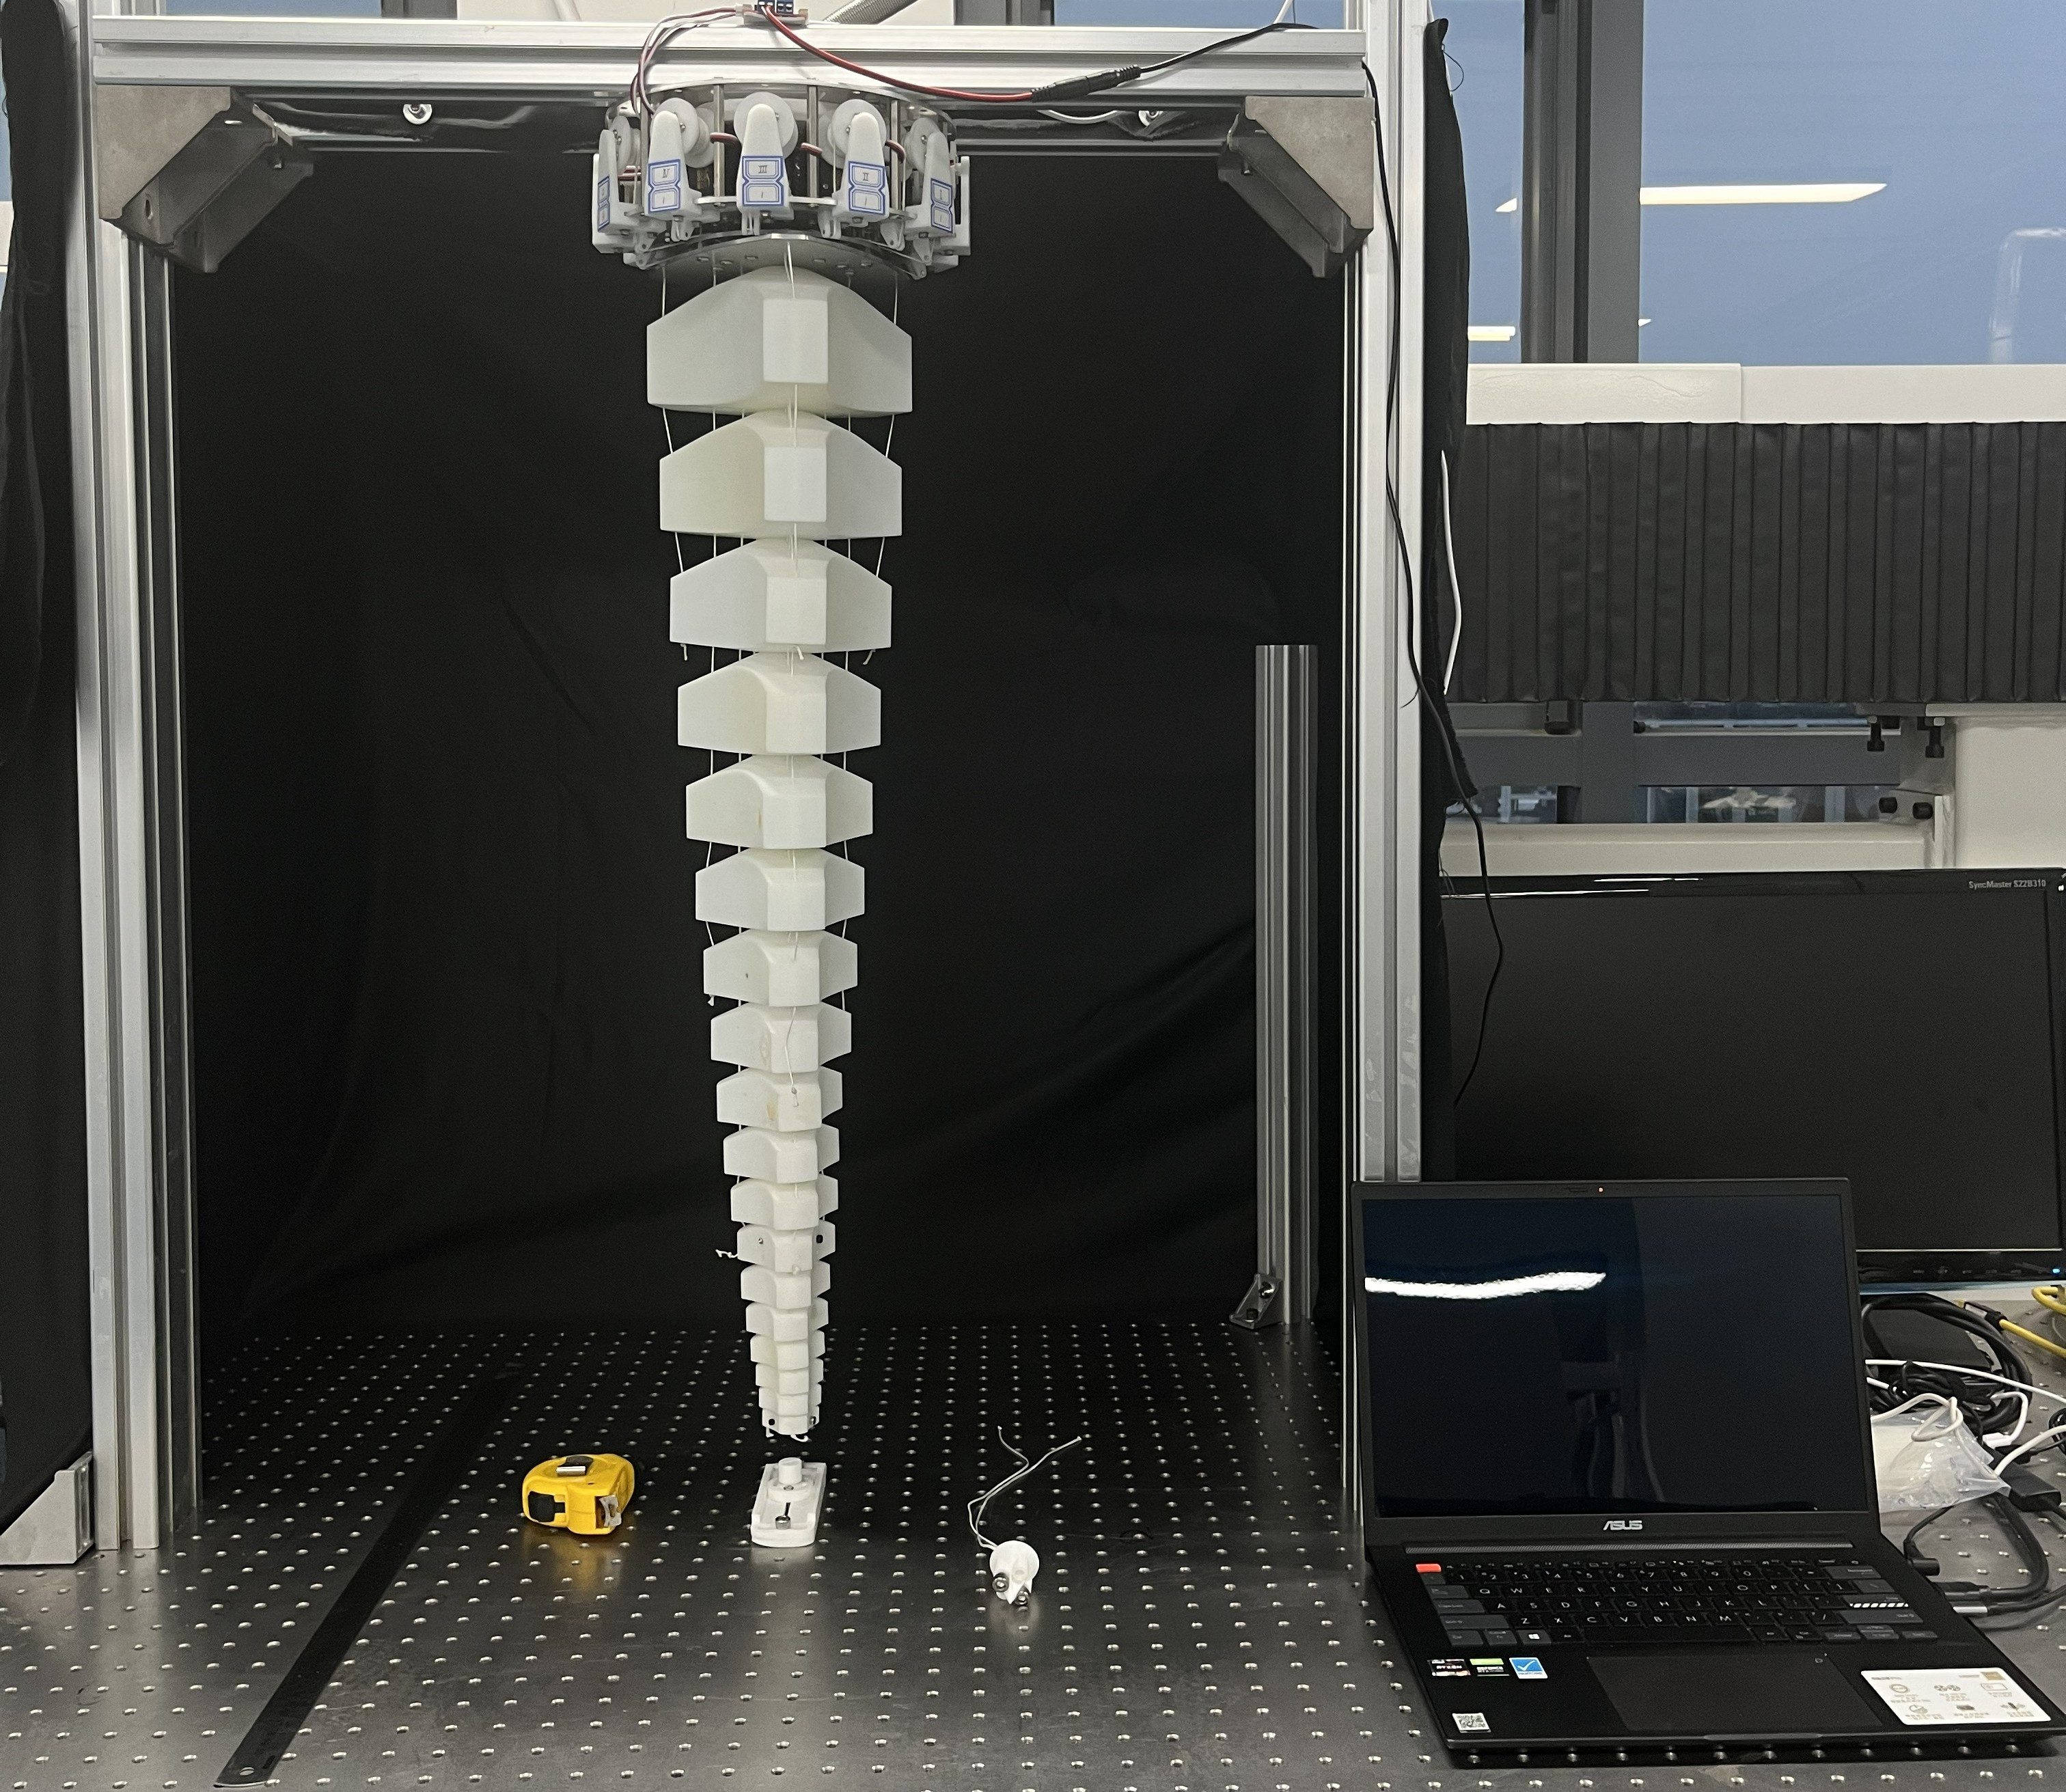
\includegraphics[width=\columnwidth]{assets/Experimental_setup.jpg}}
\caption{Preparation of experimental equipment}
\label{fig}
\end{figure}
% ===============================================

This experiment aims to quantitatively validate the accuracy of the kinematic model. The core of our setup is the robot prototype with 12 integrated servo motors (Fig. 2), which is driven by a host computer running the inverse kinematic control algorithm. We employ manual measurement methods to obtain the ground truth, using tools that include a plumb line and an industrial measuring tape.

%实验流程如下：上位机向机器人发送目标姿态指令 \texttt{{[}($\phi_1$, $\theta_1$),\ ($\phi_2$, $\theta_2$),\ ...{]}}。待机器人稳定后，我们通过铅垂线投影和卷尺测量，记录各段末端的笛卡尔坐标 $(x, y, z)$。该测量值随后被转换为圆柱坐标 \texttt{($r$,$\phi$, $z$)}，用以和正运动学模型的理论预测值进行比较。
The experimental procedure is as follows: The host computer sends a target pose command, \texttt{{[}($\phi_1$, $\theta_1$),\ ($\phi_2$, $\theta_2$),\ ...{]}}, to the robot. Once the robot stabilizes, we record the Cartesian coordinates $(x, y, z)$ of each segment's tip using plumb line projection and a measuring tape. These measured values are then converted to cylindrical coordinates \texttt{($r$,$\phi$, $z$)} for comparison with the theoretical predictions from the forward kinematic model.

% ======================================================================
%          Combination Figure 3: Demonstration of Robot Mobility
% ======================================================================
\begin{figure*}[t] % 使用 figure* 环境使其跨双栏，[t] 表示置于页面顶部
    \centering % 将整个图形环境居中
    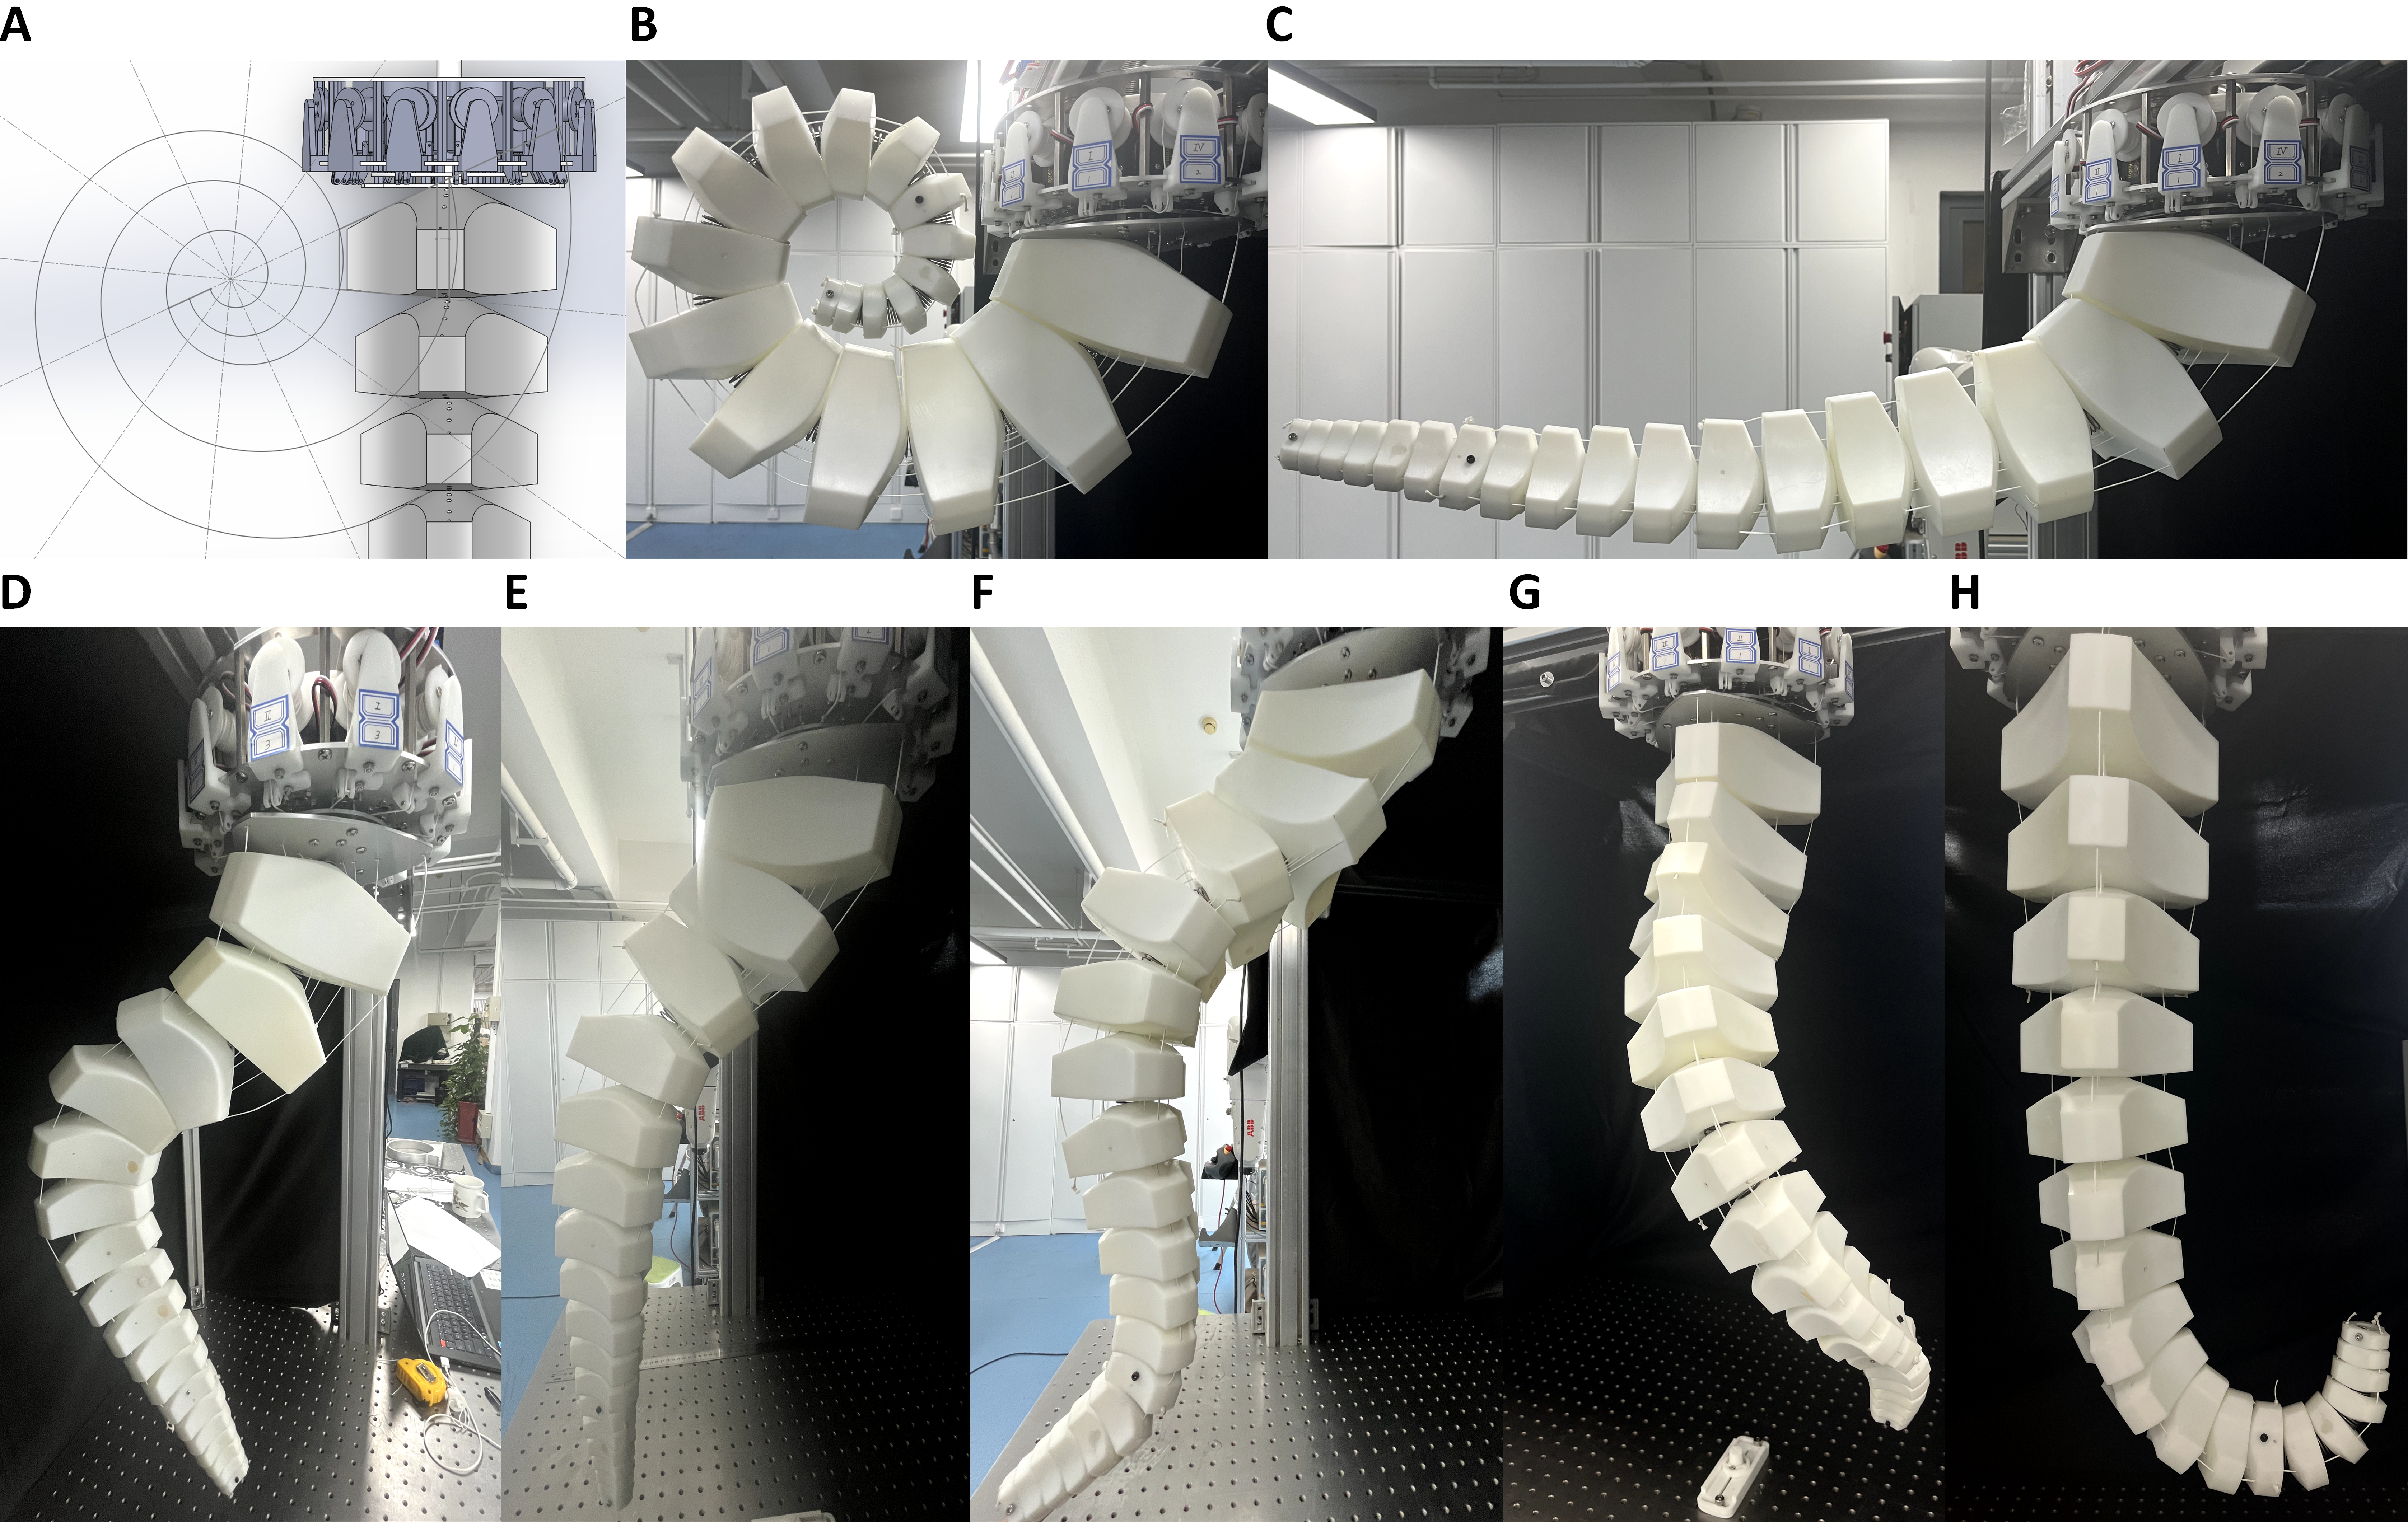
\includegraphics[width=\textwidth]{assets/All test.png}
    \caption{Demonstration of the logarithmic spiral design concept and the physical prototype's motion capabilities. (A) Design sketch; (B, C) CAD models in different bending poses; (D-H) Various complex poses achieved by the physical prototype, including C-shapes, S-shapes, and spiral bends, which showcase its extensive workspace and high flexibility.}
    \label{fig:spiral_diagram}
\end{figure*}

% ======================================================================

\subsection{Workspace and Dexterity Demonstration}
%除了定量评估，我们还进行了一系列定性实验，以直观展示机器人的运动能力。如图2所示，机器人能够完成大范围的C形弯曲(Fig. 3D, E)、灵活的S形弯曲(Fig. 3F, G)以及极具挑战性的空间螺旋姿态(Fig. 3H)，直观地展示了其超越传统刚性臂的广阔工作空间与高度灵活性。
In addition to quantitative evaluation, we conducted a series of qualitative experiments to visually demonstrate the robot's motion capabilities. As shown in Figure 3, the robot can achieve large-scale C-bends (Fig. 3D, E), flexible S-bends (Fig. 3F, G), and highly challenging spatial spiral poses (Fig. 3H). These results visually demonstrate its extensive workspace and high flexibility, which surpass those of traditional rigid arms.

%这些实验清晰地展示了： \textbf{广阔的工作空间:} 机器人能够覆盖其周围相当大的三维空间。 \textbf{高度的灵活性:} 多段独立控制与仿生结构相结合，使得机器人能够形成其他对数螺旋连续体机器人无法实现的复杂曲线。
These experiments clearly demonstrate, \textbf{Extensive Workspace:} The robot can cover a substantial three-dimensional volume around it; \textbf{High Flexibility:} The combination of independent multi-segment control and a bio-inspired structure allows the robot to form complex curves that are unachievable by other logarithmic spiral continuum robots.

% ======================================================================
%                    Summary table (Table II)
% ======================================================================
\begin{table*}[!htbp] % 建议放在页面顶部 (top)
    \captionsetup{skip=10pt}
    \centering
    \caption{Positioning Accuracy Validation for the Robot Tip (Segment 4)}
    \label{tab:summary_accuracy} % 使用一个更具描述性的标签

    % --- 使用 tabularx 环境 ---
    % \textwidth 表示表格总宽度将充满整个页面的文本宽度（跨双栏）
    % X 列类型表示该列将自动扩展并允许文本换行
    \begin{tabularx}{\textwidth}{@{} >{\RaggedRight}X c >{\centering}X >{\centering}X c @{}}
    \toprule
    % --- 表头 ---
    \textbf{ } & \textbf{Set parameters} & \textbf{Theoretical predicted position} & \textbf{Actual measurement position} & \textbf{Positioning error} \\
    \textbf{(Pose Description)} & \textbf{($\boldsymbol{\varphi}$, $\boldsymbol{\theta}$)} & \textbf{($\boldsymbol{r}$, $\boldsymbol{\varphi}$, $\boldsymbol{z}$) [mm, deg]} & \textbf{($\boldsymbol{r}$, $\boldsymbol{\varphi}$, $\boldsymbol{z}$) [mm, deg]} & \textbf{[mm]} \\
    \midrule
    
    % --- 表格数据 ---
    1 Segment: Base bend & $[(0, 90), (0,0), \dots]$ & $(694.8, 0.0, 126.0)$ & $(690, 0, 170)$ & 4.92 \\
    \addlinespace % 在行之间增加一点垂直间距，使表格更疏朗
    1 Segment: Tip bend & $[(0,0), \dots, (0, 180)]$ & $(99.2, 0.0, 653.9)$ & $(100, 0, 655)$ & 1.37 \\
    \addlinespace
    2 segments: S-shaped bend & $[(0, 60), (180, 60), \dots]$ & $(241.4, 0.0, 711.5)$ & $(165, 0, 715)$ & 76.51 \\
    \addlinespace
    2 segments: L-shaped bend & $[(90, 90), (180, 90), \dots]$ & $(562.3, 143.2, 241.4)$ & $(565, 140, 260)$ & 96.81 \\
    \addlinespace
    Space Spiral & $[(0, 50), (120, 50), \dots]$ & $(279.7, 61.3, 625.2)$ & $(250, 60, 635)$ & 31.87 \\
    \bottomrule
    \end{tabularx}
    
    % --- 表格注释 ---
    \begin{flushleft}
    \vspace{-1ex} % 稍微减少注释与表格的间距
    \footnotesize % 将注释字体设为小号
    \emph{Note: The `(0,0)` item in the parameter settings has been omitted with `...`. The positioning error is calculated as the Euclidean distance between the theoretical point converted to Cartesian coordinates and the measured point.}
    \end{flushleft}
\end{table*}
% ======================================================================

\subsection{Quantitative Model Evaluation}

%本实验旨在通过对比正运动学模型的理论预测值与物理样机的实际测量值，来验证我们整个运动学框架的有效性。我们选取了涵盖单段、双段及多段运动的18组代表性姿态进行了测试。表 II 节选并总结了其中5组最具代表性的测试结果，并计算了理论预测点与实际测量点之间的三维欧氏距离作为定位误差。
This experiment aims to validate our entire kinematic framework by comparing the theoretical predictions from the forward kinematic model against the actual measurements from the physical prototype. We tested 18 representative poses encompassing single-segment, dual-segment, and multi-segment motions. Table II selects and summarizes the five most representative test results, calculating the positioning error as the three-dimensional Euclidean distance between the predicted and measured points.

%在全部18组测试中，机器人末端执行器的\textbf{平均定位误差为 17.95 mm}，\textbf{最大误差为 96.81 mm}（出现在S形弯曲姿态下）。关键影响因素包括：（1）摩擦与回差：电缆导管中未建模的摩擦及关节处的机械回差；（2）重力与负载：纯运动学模型中未考虑的机器人自重导致的形变。
Across all 18 tests, the robot's end-effector had an \textbf{average positioning error of 17.95 mm} and a \textbf{maximum error of 96.81 mm} (which occurred in an S-shaped bending pose). Key contributing factors include: (1) \textbf{Friction and Backlash:} Unmodeled friction in the cable conduits and mechanical backlash at the joints; (2) \textbf{Gravity and Payload:} Deformation due to the robot's own weight, which is not considered in a purely kinematic model.

\subsection{Analysis and Discussion}

%实验验证了我们的设计和模型，展示了机器人在实现复杂姿态方面的高灵活性（图 3）。定量分析(表 2）表明，定位误差与姿态复杂度相关，从简单姿态的 1.37 毫米到高度耦合姿态的 96.81 毫米不等。这表明我们的运动学模型在几何上是合理的，但在复杂构型中，未建模的物理因素（如摩擦、重力）占主导地位。
The experimental results validate our design and model, demonstrating the robot's high flexibility in achieving complex poses (Fig. 3). The quantitative analysis (Table 2) reveals that the positioning error correlates with pose complexity, ranging from 1.37 mm for simple poses to 96.81 mm for highly coupled ones. This indicates that our kinematic model is geometrically sound; however, in complex configurations, unmodeled physical factors (such as friction and gravity) become the dominant source of error.

% =========================================================================
% === Section IV: Conclusions and Future Work
% =========================================================================

\section{Conclusions and Future Work}

\subsection{Conclusion}
The main contributions of our work are as follows:

\begin{enumerate}
\def\labelenumi{\arabic{enumi}.}

\item
  %进一步设计了对数螺旋连续体机器人——采用可延展的中心弹性轴结构以及实现分段驱动，实现平滑的刚度梯度变化。
  A logarithmic spiral continuum robot was designed, which features a stretchable central elastic backbone and segmental actuation to achieve a smooth stiffness gradient.
\item
  %建立了包含动态轴长补偿机制的综合耦合运动学模型，显著提升了物理真实性。
  A comprehensive coupled kinematic model was established, incorporating a dynamic backbone length compensation mechanism to significantly improve its physical realism.
\item
  %在12自由度硬件原型上进行了全面实验验证，证实了该机器人可形成复杂空间曲线，并验证了所提模型的有效性。
  Extensive experimental validation was conducted on a 12-DoF hardware prototype, confirming the robot's capability to form complex spatial curves and validating the effectiveness of the proposed model.
\end{enumerate}

%本文提出了一种新型仿生对数螺旋连续体机器人的设计、建模与实验验证。该创新展现出高灵活性与大工作空间。所提出的耦合运动学模型结合动态轴补偿机制，能有效控制机器人实现复杂空间构型。物理样机实验证实了该设计的性能，并验证了模型预测机器人形态的能力。本研究为开发适用于复杂环境的下一代连续体机器人奠定了坚实基础。
This paper presented the design, modeling, and experimental validation of a novel bio-inspired logarithmic spiral continuum robot. This innovative design exhibits high flexibility and an extensive workspace. The proposed coupled kinematic model, incorporating a dynamic backbone compensation mechanism, enables effective control of the robot to achieve complex spatial configurations. Experiments with the physical prototype have confirmed the design's performance and validated the model's predictive capability for the robot's morphology. This research provides a solid foundation for developing the next generation of continuum robots suitable for complex environments.

\subsection{Future Work}

%本研究为开发高性能连续体机器人奠定了基础，未来工作将主要围绕两个核心方向展开：提升控制精度与动态性能，以及探索面向任务的实际应用。
Our work lays the foundation for developing high-performance continuum robots. Future work will primarily revolve around two core areas: enhancing control accuracy and dynamic performance, and exploring task-oriented practical applications.

%首要任务是实现闭环控制，通过融合内部本体感知（如IMU）与外部视觉追踪，克服当前开环系统的固有局限。与此同时，我们将建立完整的动力学模型，将缆绳张力、摩擦及重力等因素纳入考量，为实现力控与环境的动态交互提供理论基础。这些控制层面的提升，将与硬件层面的设计优化和自动化标定并行，以系统性地提升模型的绝对精度。
The foremost task is to implement closed-loop control by integrating internal proprioceptive sensing (such as an IMU) with external visual tracking to overcome the inherent limitations of the current open-loop system. Concurrently, a complete dynamic model will be developed that incorporates factors like cable tension, friction, and gravity. This will provide the theoretical foundation for achieving force control and dynamic interaction with the environment. These advancements at the control level will be pursued in parallel with hardware-level design optimizations and automated calibration to systematically enhance the model's absolute accuracy.

\begin{thebibliography}{00}
\bibitem{b1} Z. Wang, N. M. Freris, and X. Wei, “SpiRobs: Logarithmic spiral-shaped robots for versatile grasping across scales,” Device, p. 100646, Dec. 2024, doi: https://doi.org/10.1016/j.device.2024.100646. 
\bibitem{b2} H. Huang et al., “Grasping by spiraling: reproducing elephant movements with rigid-soft robot synergy,” npj Robotics, vol. 3, no. 1, Jul. 2025, doi: https://doi.org/10.1038/s44182-025-00038-z.
\bibitem{b3} T. Mahl, A. Hildebrandt, and O. Sawodny, “A Variable Curvature Continuum Kinematics for Kinematic Control of the Bionic Handling Assistant,” IEEE Transactions on Robotics, vol. 30, no. 4, pp. 935–949, Aug. 2014, doi: https://doi.org/10.1109/tro.2014.2314777.
\bibitem{b4} C. A. Monje, B. Deutschmann, J. Muñoz, C. Ott, and C. Balaguer, “Fractional Order Control of Continuum Soft Robots: Combining Decoupled/Reduced-Dynamics Models and Robust Fractional Order Controllers for Complex Soft Robot Motions,” IEEE Control Systems, vol. 43, no. 3, pp. 66–99, Jun. 2023, doi: https://doi.org/10.1109/mcs.2023.3253420.
\bibitem{b5} A. Y. Alkayas, A. T. Mathew, D. Feliu-Talegon, P. Deng, T. G. Thuruthel, and F. Renda, “Soft Synergies: Model Order Reduction of Hybrid Soft-Rigid Robots via Optimal Strain Parameterization,” IEEE Transactions on Robotics, vol. 41, pp. 1118–1137, Dec. 2024, doi: https://doi.org/10.1109/tro.2024.3522182.
\bibitem{b6} K. Wu, G. Zheng, and J. Zhang, “FEM-based trajectory tracking control of a soft trunk robot,” Robotics and Autonomous Systems, vol. 150, p. 103961, Apr. 2022, doi: https://doi.org/10.1016/j.robot.2021.103961.
\bibitem{b7} R. J. Webster and B. A. Jones, “Design and Kinematic Modeling of Constant Curvature Continuum Robots: A Review,” International Journal of Robotics Research, vol. 29, no. 13, pp. 1661–1683, Nov. 2010, doi: https://doi.org/10.1177/0278364910368147.
\end{thebibliography}

% ============
% === 附录部分
% ============
% 结束正文，开始附录
\clearpage
\onecolumn

\appendices

\section{Derivation of the Single-Segment Homogeneous Transformation Matrix}
%本附录旨在详细推导正文中式(\ref{eq:T_matrix})所述的单段齐次变换矩阵 $\mathbf{T}$（为简洁，此处省略上标）。该推导基于几何分析，将弯曲段的末端位姿分解为旋转和平移的组合。
This appendix provides a detailed derivation of the single-segment homogeneous transformation matrix, $\mathbf{T}$, as presented in equation (\ref{eq:T_matrix}) of the main text (the superscript is omitted here for simplicity). The derivation is based on a geometric analysis that decomposes the tip pose of the bent segment into a combination of rotation and translation.

%假设段的起点位于坐标系 $\{S_{i-1}\}$ 的原点，段的弧长为 $L$，弯曲角度为 $\theta$，弯曲方向为 $\phi$。
It is assumed that the starting point of the segment is located at the origin of the coordinate frame $\{S_{i-1}\}$, with an arc length of $L$, a bending angle of $\theta$, and a bending direction of $\phi$.

\subsection{Translation Vector of the Tip)}
%首先，我们在一个临时的、与弯曲平面重合的 $x'-z'$ 平面内分析末端点的位置。根据圆弧几何，圆弧半径 $R = L / \theta$。末端点 $P'$ 相对于起点的坐标为：
First, the position of the tip is analyzed within a temporary $x'-z'$ plane that coincides with the bending plane. From the geometry of a circular arc, the radius of the arc is $R = L / \theta$. The coordinates of the tip, $P'$, relative to the starting point are:

\begin{align*}
    P'_x &= R(1 - \cos\theta) \\
    P'_y &= 0 \\
    P'_z &= R\sin\theta
\end{align*}

%考虑到弯曲方向 $\phi$ 是 $x'-z'$ 平面相对于 $\{S_{i-1}\}$ 的 $x-z$ 平面绕 $z$ 轴旋转 $\phi$ 角得到，因此，我们需要将 $P'$ 绕 $z$ 轴旋转 $\phi$ 角，以得到其在 $\{S_{i-1}\}$ 中的最终坐标 $P = [P_x, P_y, P_z]^T$：
Considering that the bending direction $\phi$ is obtained by rotating the $x'-z'$ plane by an angle $\phi$ about the $z$-axis relative to the $x-z$ plane of $\{S_{i-1}\}$. The point $P'$ must be rotated by $\phi$ about the $z$-axis to find its final coordinates $P = [P_x, P_y, P_z]^T$ in the $\{S_{i-1}\}$ frame:

\begin{align*}
    P_x &= P'_x \cdot \cos(\phi) = R(1 - \cos\theta)\cos\phi \\
    P_y &= P'_x \cdot \sin(\phi) = R(1 - \cos\theta)\sin\phi \\
    P_z &= P'_z = R\sin\theta
\end{align*}

%这三项构成了齐次变换矩阵的平移部分。
These three terms form the translation part of the homogeneous transformation matrix.

\subsection{Orientation of the Tip Coordinate Frame (Rotation Matrix)}
%接下来，我们确定末端坐标系 $\{S_i\}$ 的三个轴向量 $\mathbf{x}_i, \mathbf{y}_i, \mathbf{z}_i$ 在 $\{S_{i-1}\}$ 中的表示。这三个向量构成了旋转矩阵 $\mathbf{R}$ 的三列。
Next, the representations of the three axis vectors of the tip coordinate frame $\{S_i\}$—namely $\mathbf{x}_i, \mathbf{y}_i, \text{and } \mathbf{z}_i$—are determined within the $\{S_{i-1}\}$ frame. These three vectors constitute the three columns of the rotation matrix $\mathbf{R}$.

\begin{itemize}
    \item 
    % $\mathbf{z}_i$ 轴 (切线方向): $\{S_i\}$ 的 $z$ 轴是圆弧的切线方向。它是通过将 $\{S_{i-1}\}$ 的 $z$ 轴 $[0, 0, 1]^T$ 先绕 $y$ 轴旋转 $\theta$ 角，再绕 $z$ 轴旋转 $\phi$ 角得到的。
    The $\mathbf{z}_i$-axis (tangential direction): The $z$-axis of $\{S_i\}$ is tangential to the circular arc. It is obtained by first rotating the $z$-axis of $\{S_{i-1}\}$, i.e., $^T$, by an angle of $\theta$ about the $y$-axis, followed by a rotation of $\phi$ about the $z$-axis.
    \item 
    % $\mathbf{x}_i$ 轴 (法线方向): $\{S_i\}$ 的 $x$ 轴指向圆弧的圆心方向。它是通过将 $\{S_{i-1}\}$ 的 $x$ 轴 $[1, 0, 0]^T$ 进行同样的复合旋转得到的。
    The $\mathbf{x}_i$-axis (normal direction): The $x$-axis of $\{S_i\}$ points toward the center of the circular arc. This vector is obtained by applying the same sequence of rotations to the $x$-axis of $\{S_{i-1}\}$, i.e., $^T$.
    \item 
    % $\mathbf{y}_i$ 轴 (副法线方向): $\{S_i\}$ 的 y 轴始终垂直于由 $x_i$ 和 $z_i$ 定义的弯曲平面。因此，它可以通过将 $\{S_{i-1}\}$ 的 $y$ 轴 $[0, 1, 0]^T$ 绕 $z$ 轴旋转 $\phi$ 角得到，而与弯曲角度 $\theta$ 无关。
    The $\mathbf{y}_i$-axis (binormal direction): The $y$-axis of $\{S_i\}$ remains perpendicular to the bending plane defined by $\mathbf{x}_i$ and $\mathbf{z}_i$. Therefore, it can be obtained by rotating the $y$-axis of $\{S_{i-1}\}$, i.e., $^T$, by an angle of $\phi$ about the $z$-axis, and is thus independent of the bending angle $\theta$.
\end{itemize}

%将 $\mathbf{x}_i, \mathbf{y}_i, \mathbf{z}_i$ 作为列向量组合起来，便构成了与正文中式(\ref{eq:T_matrix})一致的旋转矩阵部分。
Combining $\mathbf{x}_i, \mathbf{y}_i, \text{and } \mathbf{z}_i$ as column vectors forms the rotational part of the transformation matrix, consistent with what is shown in equation (\ref{eq:T_matrix}) in the main text.

\clearpage

\section{Complete test data}

\begin{table*}[h] % [t] 建议放在页面顶部 (top) 或 [h] 尝试放在此处 (here)

% 设置标题与表格的间距，并让标题居中
\captionsetup{skip=10pt}
\centering

% 表格标题 - 已为您更新为第一段
\caption{Detailed Positioning Accuracy Data for the First Segment}
\label{tab:segment1_error_data} % 添加一个唯一的标签

% 使用 tabular 环境来创建表格，已为您更新为7列
\begin{tabular}{@{}ccccccc@{}}
\toprule
% --- 表头 ---
% 为了清晰，我们使用两行来定义表头，并用 booktabs 的 cmidrule 来画出分组线
\multicolumn{3}{c}{Theoretical Position} & \multicolumn{3}{c}{Real Position} & \\
\cmidrule(r){1-3} \cmidrule(l){4-6}
$\boldsymbol{r_{th}}$ (mm) & $\boldsymbol{\varphi_{th}}$ (deg) & $\boldsymbol{z_{th}}$ (mm) & $\boldsymbol{r_{r}}$ (mm) & $\boldsymbol{\varphi_{r}}$ (deg) & $\boldsymbol{z_{r}}$ (mm) & Error (mm) \\
\midrule
% --- 表格数据 ---
% 我已将您图片中的19行数据精确地转录到这里
170.95 & 0 & 170.95 & 170 & 0 & 170 & 1.34 \\
164.41 & 0 & 179.42 & 165 & 0 & 180 & 0.83 \\
95.66  & 0 & 230.94 & 95  & 0 & 230 & 1.15 \\
0      & 0 & 244.48 & 0   & 0 & 245 & 0.52 \\
0      & 0 & 244.48 & 0   & 0 & 245 & 0.52 \\
0      & 0 & 244.48 & 0   & 0 & 245 & 0.52 \\
0      & 0 & 244.48 & 0   & 0 & 245 & 0.52 \\
0      & 0 & 244.48 & 0   & 0 & 245 & 0.52 \\
0      & 0 & 244.48 & 0   & 0 & 245 & 0.52 \\
0      & 0 & 244.48 & 0   & 0 & 245 & 0.52 \\
0      & 0 & 244.48 & 0   & 0 & 245 & 0.52 \\
64.61  & 0 & 241.12 & 65  & 0 & 240 & 1.19 \\
124.39 & 0 & 215.44 & 115 & 0 & 210 & 10.85 \\
170.95 & 90& 170.95 & 165 & 90& 175 & 7.20 \\
157.34 & 0 & 187.51 & 115 & 0 & 210 & 47.94 \\
115.13 & 0 & 221.17 & 115 & 0 & 210 & 11.17 \\
0      & 0 & 244.48 & 0   & 0 & 240 & 4.48 \\
157.34 & 0 & 187.51 & 155 & 0 & 185 & 3.43 \\
0      & 0 & 244.48 & 0   & 0 & 245 & 0.52 \\
124.39 & 0 & 215.44 & 125 & 0 & 215 & 0.75 \\
105.54 & 0 & 226.34 & 10  & 0 & 225 & 95.55 \\
164.41 & 0 & 179.42 & 165 & 0 & 180 & 0.83 \\
\bottomrule
\end{tabular}

% 设置标题与表格的间距，并让标题居中
\captionsetup{skip=10pt}
\centering

% 表格标题 - 已为您更新为第二段
\caption{Detailed Positioning Accuracy Data for the Second Segment}
\label{tab:segment2_error_data} % 为第二段的表格设置一个唯一的标签

% 使用 tabular 环境来创建表格
\begin{tabular}{@{}ccccccc@{}}
\toprule
% --- 专业表头 ---
\multicolumn{3}{c}{Theoretical Position} & \multicolumn{3}{c}{Real Position} & \\
\cmidrule(r){1-3} \cmidrule(l){4-6}
$\boldsymbol{r_{th}}$ (mm) & $\boldsymbol{\varphi_{th}}$ (deg) & $\boldsymbol{z_{th}}$ (mm) & $\boldsymbol{r_{r}}$ (mm) & $\boldsymbol{\varphi_{r}}$ (deg) & $\boldsymbol{z_{r}}$ (mm) & Error (mm) \\
\midrule
% --- 表格数据 ---
% 我已将您图片中的21行数据精确地转录到这里
401.49 & 0      & 170.95 & 400 & 0   & 185 & 14.13 \\
394.07 & 0      & 199.51 & 395 & 0   & 200 & 1.05 \\
258.67 & 0      & 393.95 & 255 & 0   & 390 & 5.39 \\
186.02 & 180    & 351.88 & 185 & 180 & 355 & 3.28 \\
183.23 & 180    & 361.21 & 185 & 180 & 360 & 2.14 \\
117.04 & 180    & 447.21 & 115 & 180 & 445 & 3.01 \\
0      & 0      & 475.02 & 0   & 0   & 475 & 0.02 \\
0      & 0      & 475.02 & 0   & 0   & 475 & 0.02 \\
0      & 0      & 475.02 & 0   & 0   & 475 & 0.02 \\
0      & 0      & 475.02 & 0   & 0   & 475 & 0.02 \\
0      & 0      & 475.02 & 0   & 0   & 475 & 0.02 \\
0      & 0      & 475.02 & 0   & 0   & 475 & 0.02 \\
267.33 & 0      & 358.16 & 265 & 0   & 360 & 2.97 \\
241.43 & 0      & 418.17 & 165 & 0   & 430 & 77.34 \\
368.54 & 115.85 & 170.95 & 370 & 115 & 210 & 39.46 \\
332.21 & 24.77  & 294.55 & 360 & 20  & 275 & 44.53 \\
303.98 & 0      & 353.40 & 315 & 0   & 320 & 35.17 \\
117.04 & 0      & 447.21 & 115 & 0   & 430 & 17.33 \\
355.82 & 0      & 313.96 & 340 & 0   & 310 & 16.31 \\
0      & 0      & 475.02 & 5   & 0   & 470 & 7.09 \\
193.19 & 0      & 433.66 & 190 & 0   & 425 & 9.23 \\
251.96 & 19.97  & 401.34 & 180 & 20  & 390 & 72.85 \\
296.67 & 0      & 7.06   & 295 & 0   & 5   & 2.65 \\
\bottomrule
\end{tabular}

\end{table*}

\begin{table*}[t] % 将表格置于页面顶部

% 设置标题与表格的间距，并让标题居中
\captionsetup{skip=10pt}
\centering

% 表格标题 - 已为您更新为第三段
\caption{Detailed Positioning Accuracy Data for the Third Segment}
\label{tab:segment3_error_data} % 为第三段的表格设置一个唯一的标签

% 使用 tabular 环境来创建表格
\begin{tabular}{@{}ccccccc@{}}
\toprule
% --- 专业表头 ---
\multicolumn{3}{c}{Theoretical Position} & \multicolumn{3}{c}{Real Position} & \\
\cmidrule(r){1-3} \cmidrule(l){4-6}
$\boldsymbol{r_{th}}$ (mm) & $\boldsymbol{\varphi_{th}}$ (deg) & $\boldsymbol{z_{th}}$ (mm) & $\boldsymbol{r_{r}}$ (mm) & $\boldsymbol{\varphi_{r}}$ (deg) & $\boldsymbol{z_{r}}$ (mm) & Error (mm) \\
\midrule
% --- 表格数据 ---
% 我已将您图片中的23行数据精确地转录到这里
580.36 & 0      & 170.95 & 580 & 0   & 185 & 14.05 \\
572.26 & 0      & 215.10 & 570 & 0   & 215 & 2.26 \\
385.15 & 0      & 520.43 & 385 & 0   & 520 & 0.46 \\
340.92 & 180    & 262.44 & 345 & 180 & 270 & 8.59 \\
345.34 & 180    & 285.62 & 345 & 180 & 285 & 0.71 \\
271.95 & 180    & 536.64 & 270 & 180 & 535 & 2.55 \\
153.27 & 90     & 516.09 & 155 & 90  & 520 & 4.28 \\
153.70 & 90     & 523.48 & 155 & 90  & 525 & 2.00 \\
111.52 & 90     & 620.35 & 110 & 90  & 620 & 1.56 \\
0      & 0      & 653.89 & 0   & 0   & 655 & 1.11 \\
0      & 0      & 653.89 & 0   & 0   & 655 & 1.11 \\
0      & 0      & 653.89 & 0   & 0   & 655 & 1.11 \\
446.20 & 0      & 358.16 & 445 & 0   & 360 & 2.20 \\
241.43 & 0      & 597.04 & 165 & 0   & 600 & 76.49 \\
474.66 & 135.68 & 170.95 & 475 & 135 & 245 & 74.26 \\
410.30 & 45.79  & 382.63 & 410 & 40  & 370 & 43.31 \\
487.24 & 0      & 377.53 & 460 & 0   & 355 & 35.35 \\
301.66 & 0      & 447.21 & 295 & 0   & 460 & 14.42 \\
458.41 & 0      & 460.48 & 430 & 0   & 470 & 29.96 \\
127.68 & 90     & 602.70 & 115 & 85  & 590 & 20.83 \\
291.76 & 0      & 574.43 & 330 & 0   & 510 & 74.92 \\
295.70 & 46.74  & 529.02 & 210 & 45  & 535 & 86.24 \\
138.60 & 0      & 20.89  & 135 & 0   & 20  & 3.71 \\
\bottomrule
\end{tabular}

% 设置标题与表格的间距，并让标题居中
\captionsetup{skip=10pt}
\centering

% 表格标题 - 已为您更新为第四段
\caption{Detailed Positioning Accuracy Data for the Fourth Segment (End-Effector)}
\label{tab:segment4_error_data} % 为第四段的表格设置一个唯一的标签

% 使用 tabular 环境来创建表格
\begin{tabular}{@{}ccccccc@{}}
\toprule
% --- 专业表头 ---
\multicolumn{3}{c}{Theoretical Position} & \multicolumn{3}{c}{Real Position} & \\
\cmidrule(r){1-3} \cmidrule(l){4-6}
$\boldsymbol{r_{th}}$ (mm) & $\boldsymbol{\varphi_{th}}$ (deg) & $\boldsymbol{z_{th}}$ (mm) & $\boldsymbol{r_{r}}$ (mm) & $\boldsymbol{\varphi_{r}}$ (deg) & $\boldsymbol{z_{r}}$ (mm) & Error (mm) \\
\midrule
% --- 表格数据 ---
% 我已将您图片中的23行数据精确地转录到这里
694.83 & 0      & 170.95 & 690 & 0   & 170 & 4.92 \\
686.30 & 0      & 225.08 & 685 & 0   & 225 & 1.30 \\
466.10 & 0      & 601.37 & 465 & 0   & 600 & 1.76 \\
440.06 & 180    & 205.21 & 440 & 180 & 215 & 9.79 \\
449.09 & 180    & 237.24 & 450 & 180 & 235 & 2.42 \\
371.08 & 180    & 593.88 & 370 & 180 & 595 & 1.56 \\
210.50 & 90     & 416.95 & 215 & 90  & 425 & 9.22 \\
219.36 & 90     & 429.71 & 220 & 90  & 430 & 0.70 \\
222.09 & 90     & 649.98 & 220 & 90  & 650 & 2.09 \\
99.20  & 0      & 653.89 & 100 & 0   & 655 & 1.37 \\
101.09 & 0      & 658.30 & 100 & 0   & 660 & 2.02 \\
86.04  & 0      & 739.93 & 85  & 0   & 740 & 1.04 \\
560.67 & 0      & 358.16 & 560 & 0   & 360 & 1.96 \\
241.43 & 0      & 711.51 & 165 & 0   & 715 & 76.51 \\
562.27 & 143.85 & 170.95 & 565 & 140 & 260 & 96.81 \\
480.51 & 54.92  & 438.99 & 460 & 55  & 440 & 20.55 \\
594.80 & 0      & 338.37 & 575 & 0   & 310 & 34.60 \\
400.80 & 0      & 389.97 & 390 & 0   & 370 & 22.70 \\
524.07 & 0      & 554.25 & 510 & 0   & 570 & 21.12 \\
213.72 & 90     & 516.67 & 190 & 85  & 510 & 30.27 \\
405.79 & 0      & 564.45 & 440 & 0   & 570 & 34.66 \\
279.66 & 61.38  & 625.24 & 250 & 60  & 635 & 31.87 \\
233.05 & 0      & 87.03  & 230 & 0   & 85  & 3.66 \\
\bottomrule
\end{tabular}

\end{table*}

\end{document}
